\section{Zielsetzung}
\label{sec:Zielsetzung}
Es wird eine $\gamma$-Strahler verwendet um durch Tomographie die Zusammensetzung eines Würfels zu untersuchen.
Dazu werden aus verschiedenen Positionen die Absorptionsspektren aufgezeichnet.

\section{Theorie}
\label{sec:Theorie}

\subsection{Wechselwirkung von \texorpdfstring{$\gamma$}{gamma}-Quanten mit Materie}
\label{sec:WW}
Ein $\gamma$-Quanten verliert nach jeder Wechselwirkung einen Teil seiner ursprünglichen Energie, bis die gesamte Energie im Absorber deponiert wird oder das $\gamma$-Quant heraus gestreut wird.
Die Teilchenzahl des $\gamma$-Strahls und damit die Intensität
\begin{equation}
  \label{eq:Absorbtion}
  I(D)=I_0\exp(-\sum_i \mu_\text{i} D_\text{i})
\end{equation}
hängt von der Schichtdicken $D_\text{i}$ der Absorber und den Extinktionskoeffizienten $\mu_\text{i}$ ab. 
Misst man nun die Intensität $I(D)$ nach Durchdringen eines Materials mit bekannter Dicke $D$ und ist die Eingangsintensität $I_0$ bekannt, so ergibt sich ein lineares 
Gleichungssystem.
Bei $\gamma$-Strahlung treten hauptsächlich die Wechselwirkungen Photoeffekt, Compton-Effekt und Paarbildung auf.

\subsubsection{Photoeffekt}
\label{sec:PhEffekt}
Dieser Effekt tritt auf, wenn das $\gamma$-Quant eine höhere Energie als die Bindungsenergie des Elektrons besitzt.
Die Energie des $\gamma$-Quants löst ein Elektron aus der Elektronenhülle, welches jetzt die Energie $E_\gamma-E_{\symup{e}}$ besitzt.
Das Loch in der K-Schale wird von einem Elektron aus einer höheren Schale aufgefüllt, das Loch in der höheren Schale wird von einem Elektron aus der Schale darüber gefüllt usw.
Die freigewordene Energie wird in Form von charakteristischen Röntgenquanten freigesetzt.
Diese $\gamma$-Quanten können den Absorber nicht verlassen und deponieren ihre gesamte Energie im Material.
Der Wirkungsquerschnitt des Photoeffekts
\begin{equation*}
\sigma_{Ph}\propto Z^\alpha E^\delta
\end{equation*}
ist stark von der Kernladungszahl $Z$ und der Energie der $\gamma$-Quanten abhängig, wobei $\num{4}<\alpha<\num{5}$ und $\delta\approx \num{-3.5}$ für natürliche Strahler gilt.

\subsubsection{Compton-Effekt}
\label{sec:ComEffekt}
Der Compton-Effekt beschreibt die elastische Streuung des $\gamma$-Quants an einem quasi freien punktförmigen Elektron, wobei das $\gamma$-Quant einen Teil seiner Energie an das Elektron abgibt.
Der Prozess ist in Abbildung \ref{fig:Compton} zu sehen.
Die Energie nach der Streuung bestimmt sich aus
\begin{equation}
E_{\gamma'}=E_{\gamma}\frac{1}{1+\frac{E_{\gamma}}{m_{\symup{e}} c^2}(1-\cos(\Psi_{\gamma}))}.
\end{equation}
Hier ist $m_{\symup{e}}$ die Masse des Elektrons, $c$ die Lichtgeschwindigkeit und $\Psi_{\gamma}$ der Streuwinkel des gestreuten $\gamma$-Quants.
Das eintreffende $\gamma$-Quant kann also nicht seine gesamte Energie an das Elektron übertragen.
Der maximale Übertrag tritt bei einem Streuwinkel von \SI{180}{\degree} auf und wird Rückstreuung genannt.
 \begin{figure}
   \centering
   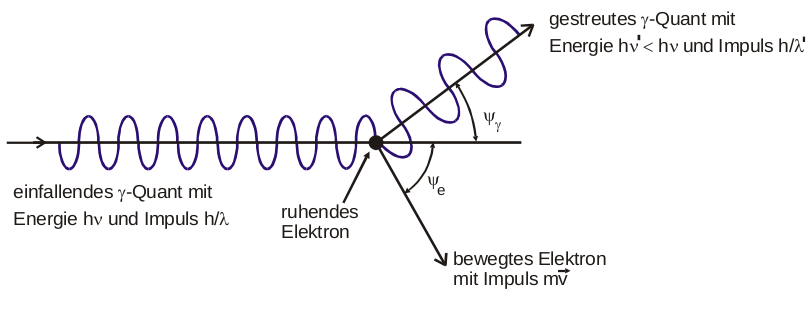
\includegraphics[height=5.5cm]{content/pictures/Compton.png}
   \caption{Der Compton-Streuprozesses schematisch dargestellt.\cite{V18}}
   \label{fig:Compton}
 \end{figure}

\subsubsection{Paarbildung}
\label{sec:Paar}
Bei der Paarbildung wandelt sich das $\gamma$-Quant in ein Elektron und ein Positron um, falls es die dafür nötige Energie $E_{\gamma}>2m_{\symup{e}}c^2$ besitzt.
Damit dieser Prozess (vom Ruhesystem des $\gamma$-Quants aus gesehen) stattfinden kann, muss zusätzlich noch ein Stoßpartner vorhanden sein.
Ist dieser Partner ein Elektron, benötigt das $\gamma$-Quant aufgrund der Rückstoßenergie sogar die vierfache Ruhemasse des Elektrons an Energie, damit es zur Paarbildung kommen kann.
Der Wirkungsquerschnitt $\sigma_{\symup{Pa}}$ ist je nach Ort, an dem die Paarerzeugung stattfindet, unterschiedlich groß, da zum Beispiel im Bereich der K-Schale das gesamte Coulomb-Feld mitwirkt, bei äußeren Schalen
jedoch Abschirmungseffekte eine Rolle spielen, wodurch $\sigma_{\symup{Pa}}$ von der Abschirmung abhängt.

\subsection{Tomographie}
\label{sec:Tomo}
Unter Tomographie wird ein bildgebendes Verfahren, welches einzelne Schichten auflöst bezeichnet. Durch mehrer solcher Bilder kann dann ein räumliches 
Abbild geschaffen werden. Dazu sind mehrer Messungen notwendig, dies soll hier bei einem 
Würfel, welcher aus \num{27} einzelnen Würfeln zusammengestzt ist untersucht werden, dabei sind die unterschiedlichen Dichten ausschlaggebend.
Wird aus der Messung der Intensität ohne Probe $I_0$ und mit Probe $I_\text{i}$ das logarithmische Verhältnis
\begin{equation}
    \label{eqn:Verhältnis}
    \ln\left(\frac{I_0}{I_\text{i}}\right) = \sum_i \mu_\text{i} d_\text{i} = N_\text{i}
\end{equation}
bestimmt, so lässt sich darauß das lineare Gleichungssystem lösen. Werden nun mehr Messungen als die \num{9} in einer Ebene befindenden Würfel durchgeführt, 
so ergibt sich ein überbestimmtes Gleichungssystem der Ordnung $m$, wenn $m$ die Anzahl durchgeführter Messungen ist.
Das Gleichungssystem lässt sich nun nach
\begin{equation}
    \label{eqn:Gleichungssystem}
    \textbf{A} \vec{\mu} = \vec{N}
\end{equation}
bestimmen, wobei $\vec{\mu} = (\mu_1, \ldots,\mu_9)^\text{T}$ der Spaltenvektor der \num{9} Absorbtionskoeffizenten und $\vec{N} = (N_1, \ldots,N_m)^\text{T}$ ist. 
\textbf{A} enthält nun die Informationen über die Anordnung der Würfel und ist eine $9 \times m$-Matrix. Werden alle Messungen mit gleicher Unsicherheit 
aufgenommen so ergeben sich die Absorbtionskoeffizenten nach
\begin{equation}
    \label{eqn:Absorbtionskoeffizenten}
    \vec{\mu} = (\textbf{A}^\text{T} \textbf{A})^{-1} \cdot \textbf{A}^\text{T} \vec{N},
\end{equation}
mit der Unsicherheit von
\begin{equation}
    \label{eqn:Unsicherheit}
    \sigma = \sqrt{\text{diag}[(\textbf{A}^\text{T} \textbf{A})^{-1}]}.
\end{equation}
Es ist zu beachten, dass die Absorbtionskoeffizenten $\mu_\text{i}$ keine Konstanten sind, sondern auch von der verwendeten Energie abhängig sind. 
Da natürliche Strahler für die Unersuchung verwendet werden, ist es wichtig ihr Energiespektrum zu kennen. Ein Energiespektrum ensteht durch Auftragen der 
Intensität oder Zählrate nach dem Durchgang einer bekannten Probe gegen die Energie. Das Spektrum für den hier verwendeten \ce{^137Cs}-Strahler ist in Abbildung \ref{fig:spektrum} zu finden.
Es sind die Charakteristiker des Compton-Kontinuums für kleine Energien bis hin zur Compton-Kante, an der das $\gamma$-Quant zurück geworfen wird, zu erkennen. 
Ebenso lässt sich deutlich der Vollenergiepeak, welcher durch den Photo-Effekt dominiert wird zu erkennen. Wird die Wellenlänge noch kleiner, so tritt die Paarerzeugung
in Erscheinung und die Intensität steigt wieder an.

 \begin{figure}
   \centering
   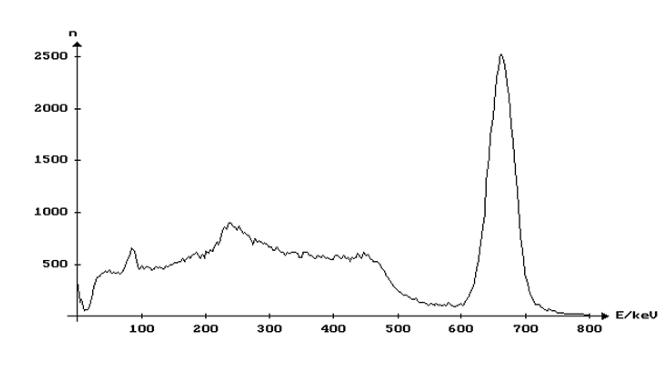
\includegraphics[height=5.5cm]{content/pictures/Spektrum.png}
   \caption{Das Energie Spektrum des verwendeten Cäsium Strahlers.\cite{spektrum}}
   \label{fig:spektrum}
 \end{figure}